% suivi.tex
% 
% author : abisutti
% created : Mon, 19 Oct 2015 13:48:21 +0200
% modified : Mon, 19 Oct 2015 13:48:21 +0200



\documentclass[xcolor=dvipsnames]{beamer}

\usepackage[T1]{fontenc}
\usepackage[utf8]{inputenc}
\usepackage[francais]{babel}
\usepackage{array}
\usepackage{tabularx}
\usepackage{multirow}
\usepackage{textcomp}
\usepackage{xstring}
\usepackage{hyperref}
\usepackage{pifont}

%%% MACRO %%%


% FIXME Prendre en compte les majuscule déjà présente
\makeatletter
\@ifpackageloaded{xstring}{
	\newcommand\smallcaps[1]{\StrLeft{#1}{1}\scriptsize\uppercase{\StrGobbleLeft{#1}{1}}\normalsize }
}{
	\newcommand\smallcaps[1]{\textsc{#1}}
}
\makeatother



%===============================================================================
% Définit un type de puce pour une liste. Si le pakage "pifont" est chargé, il 
% est utilisé, sinon on met un tiret.
\makeatletter
\@ifpackageloaded{pifont}{
	\newcommand\goodItemArrow[0]{\ding{226}}
}{
	\newcommand\goodItemArrow[0]{-}
}
\makeatother



%===============================================================================
% Item de liste avec spécification de la puce et paramètre écrit en gras.
\newcommand\functionality[1]{
	\item[\goodItemArrow] \textbf{#1}\\
}



%===============================================================================
% Commande \Euro indépendante des paquets chargés 
\makeatletter
\@ifpackageloaded{eurosym}{
	\newcommand\Euro[0]{\euro{}}
}{
	\@ifpackageloaded{textcomp}{
		\newcommand\Euro[0]{\texteuro}
	}{
		\newcommand\Euro[0]{Euro}
	}
}
\makeatother



%===============================================================================
% Accès à des variables dans le document. 
%\makeatletter
%\let\titleName\@title
%\let\subtitleName\@subtitle
%\let\authorName\@author
%\makeatother



% Titre de la section courante (que dans beamer)
%\secname 
% Titre de la sous-section courante (que dans beamer)
%\subsecname





\title[Revue de projet]{Surfaces de r\'evolution discrètes}
\subtitle{Revue de projet}
\author[]{Zied \smallcaps{Ben} \smallcaps{Othmane} \\ Thomas \smallcaps{Benoist}
	\\ Adrien \smallcaps{Bisutti} \\ Lydie \smallcaps{Richaume}}
\institute{Universit\'e de Poitiers}
\date{3 Février 2016}


\usetheme{Madrid}
\usecolortheme{sidebartab}
\usefonttheme{professionalfonts}

\definecolor{fondtitre}{rgb}{0.0,0.35,0.7}
\setbeamercolor{palette primary}{bg=fondtitre}
\setbeamercolor{palette secondary}{bg=fondtitre!75!black}
\setbeamercolor{palette tertiary}{bg=fondtitre!55!black}
\setbeamercolor{palette quaternary}{bg=fondtitre!35!black}
\setbeamercolor{item}{fg=fondtitre}

%%% MACRO %%%


% Vide la barre de navigation
\setbeamertemplate{navigation symbols}{}


% Affichage du plan à chaque début de section
\AtBeginSection[]{
	\begin{frame}{Plan}
		\begin{columns}
			\begin{column}{5cm}
			  	\tableofcontents[sections={1-3}, currentsection, hideothersubsections]
			\end{column}
			\begin{column}{5cm}
			  	\tableofcontents[sections={4-7}, currentsection, hideothersubsections]
			\end{column}
		\end{columns}
	\end{frame}
}



%%% DOCUMENT %%%

\begin{document}



%===============================================================================
%	TITRE
%===============================================================================


\begin{frame}
	\titlepage
	
\includegraphics[width=2cm]{../Images/logo-Xlim.png}
	\hfill
	
\includegraphics[width=2cm]{../Images/logo_univ_poitiers.png}
\end{frame}



%===============================================================================
%	INTRODUCTION
%===============================================================================

\section{Introduction}

% --- Contexte -----------------------------------------------------------------
	\subsection{Contexte}
	\begin{frame}{\subsecname}
		\begin{itemize}
			\item Nouvel algorithme conçu par \'Eric \smallcaps{Andres} et
				Ga\"elle \smallcaps{Largeteau}-\smallcaps{Skapin} pour mod\'eliser
				des surfaces de r\'evolution discr\`etes.
			\item Visualisation des r\'esultats avec Mathematica
		\end{itemize}
		\begin{figure}
			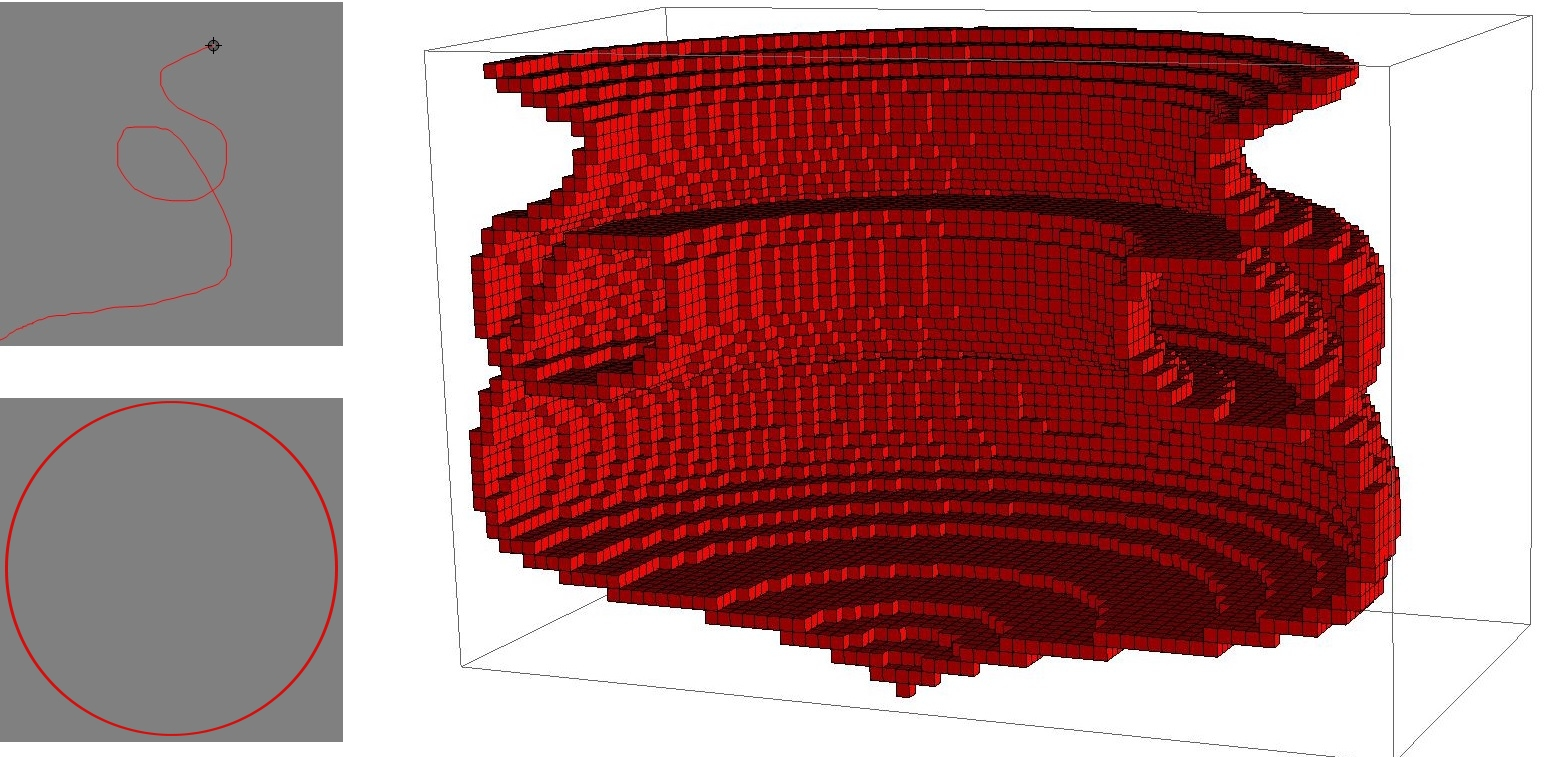
\includegraphics[height=3.8cm]{../Images/revolution2.jpg}
		\end{figure}
		\begin{itemize}
			\item Besoin d'un outil utilisable partout et par tous
		\end{itemize}
	\end{frame}


% --- Contexte -----------------------------------------------------------------
	\subsection{Objectifs}
	\begin{frame}{\subsecname}
		\begin{itemize}
			\item Objectifs métiers
			\begin{itemize}
				\item Illustrer les r\'esultats de l'algorithme
				\item Mettre \`a disposition un outil de mod\'elisation
			\end{itemize}
		\end{itemize}
		\begin{itemize}
			\item Objectifs techniques
			\begin{itemize}
				\item Application web $\to$ WebGL
				\item Utilisable par tous
			\end{itemize}
		\end{itemize}
	\end{frame}



%===============================================================================
%	DEROULEMENT
%===============================================================================

\section{Planification}

% --- Taches -------------------------------------------------------------------
	\subsection{T\^aches} % FIXME Checked or not with \ding{52} and \ding{56} of pifont
	\newcommand{\Valid}{{\color{ForestGreen}\ding{52}}}
	\newcommand{\notCheck}{{\color{BrickRed}\ding{56}}}
	\begin{frame}{\subsecname}
		\begin{center}
		{\renewcommand{\arraystretch}{1.3}
		\begin{tabular}{|m{4.5cm}<{\centering}c|m{4.5cm}<{\centering}c|}
			\hline
			\multicolumn{3}{|c}{1 - Documentation, test et aide utilisateur} & \notCheck\\
			\hline
			\multicolumn{3}{|c}{2 - Conception} & \Valid\\
			\hline
			\centering
			3 - Noyau fonctionnel & \Valid & 4 - Interface minimale & \Valid\\
			\hline
			6 - Ajout de fonctionnalités & \Valid & 5 - Am\'elioration IHM \linebreak Choix des courbes & \Valid\\
			\hline
			8 - Dessin \`a main levée m\'eridienne & \notCheck & 7 - Am\'elioration IHM Param\`etres & \Valid\\
			\hline
			9 - Gestion des donn\'ees & \notCheck & 10 - Am\'elioration IHM \linebreak Rentrer des formules & \notCheck\\
			\hline
			\multicolumn{3}{|c}{11 - Ajout courbes utilisateur} & \notCheck\\
			\hline
			\multicolumn{3}{|c}{12 - R\'edaction rapport technique} & \notCheck\\
			\hline
		\end{tabular}}
		\end{center}
	\end{frame}

	
%===========================================================================================
%	Organisation
%===========================================================================================


% --- Gantt --------------------------------------------------------------------
	\subsection{Gantt}
	\begin{frame}{\subsecname}
		\begin{center}
			\href{run:./Images/Gantt_ProjetDiscret.gif}{Diagramme pr\'evisionnel}\\
			\bigskip
			\href{run:Images/Gantt_ProjetDiscretRéférence.gif}{Diagramme pr\'evisionnel r\'evis\'e}
		\end{center}
	\end{frame}

	
% --- Zoom Gantt Initial --------------------------------------------------------------------
	\begin{frame}{Gantt (zoom)}
		\begin{center}
			\href{run:Images/GantInitialClasses.gif}{Zoom diagramme pr\'evisionnel}\\
			\bigskip
			\href{run:Images/GantReferenceClasses.gif}{Zoom diagramme prévisionnel révisé}
		\end{center}
	\end{frame}

	
% --- Gantt --------------------------------------------------------------------
	\subsection{Gantt de suivi}
	\begin{frame}{\subsecname}
		\begin{center}
			\href{run:Images/Gantt_ProjetDiscretSuivi2.gif}{Diagramme de suivi}
		\end{center}
	\end{frame}


% --- Avancement ---------------------------------------------------------------
	\subsection{Avancement}
	\begin{frame}{\subsecname}
		\begin{figure}
			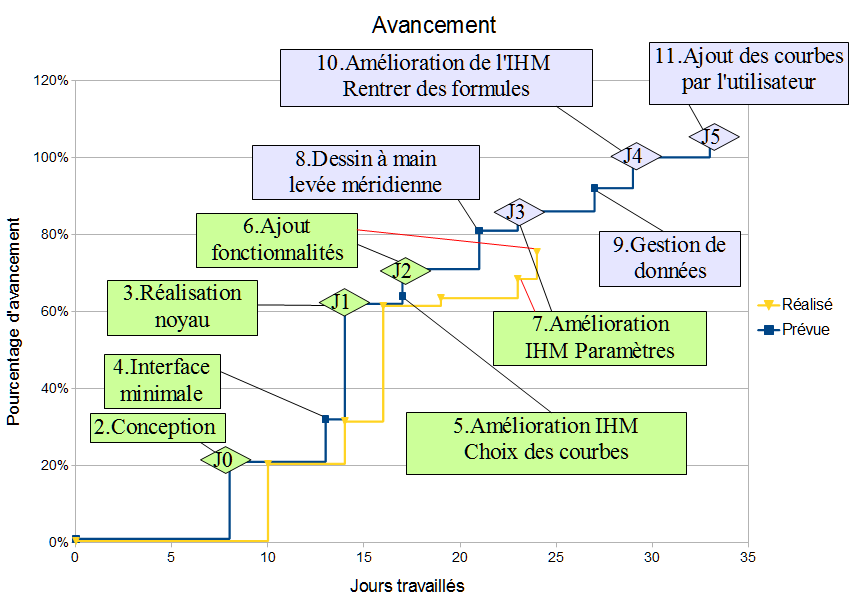
\includegraphics[height=7cm]{Images/Avancement.png}
		\end{figure}
	\end{frame}


% --- Avancement ---------------------------------------------------------------
	\begin{frame}{\subsecname}
		\begin{figure}
			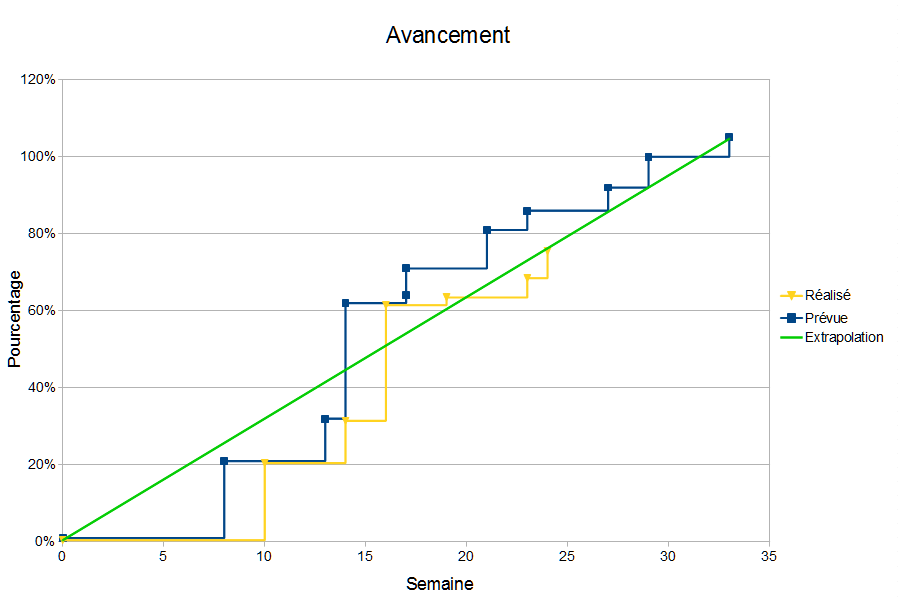
\includegraphics[height=6cm]{Images/Avancement2.png}
		\end{figure}
		% FIXME table 3 colones
		\begin{tabular}{ll}
		Avancement moyen pr\'evisionnel\,\,\,\,: & 3,18 \%/jour (3,74 sur la p\'eriode)\\
		Avancement moyen observ\'e\,\,\,: & 3,13 \%/jour
		\end{tabular}
	\end{frame}


% --- Livrables ----------------------------------------------------------------
	\subsection{Livrables}
	\begin{frame}{\subsecname}
		\begin{center}
		\small
		\begin{tabular}{|c|>{\raggedright}m{3cm}|c|c|c|}
			\hline
			\textbf{\No} & \textbf{Livrable} & \textbf{T\^aches}
			& \textbf{Date pr\'evue} & \textbf{Date effective}\\
			\hline
			1 & R\'esultat de l'algorithme et interface & 2, 3, 4 & 23/12 
			& 18/01\\
			\hline
			2 & Application minimale & 5, 6 & 21/01 & 25/01\\
			\hline
			2\textsuperscript{bis} & Multicoupe et param\`etres & 7 & --- & 29/01\\
			\hline
			3 & Courbes avec param\`etres modifiables et trac\'e \`a main
			lev\'ee& 7, 8 & 29/01 & ---\\
			\hline
			4 & \'Equations et export & 9, 10 & 19/02 & ---\\
			\hline
			5 & Application finale et documentation & 11 & 02/03 & ---\\
			\hline
		\end{tabular}
		\end{center}
	\end{frame}



%===============================================================================
%	DEMO
%===============================================================================

\section{D\'emonstration}

\begin{frame}{\secname}
	\begin{figure}
		\href
		{run:../../../ApplicationDiscret/Application/discreteSurface.html}
		{D\'emonstration}
	\end{figure}
\end{frame}



%===============================================================================
%	RISQUES
%===============================================================================

\section{\'Evolution des risques}


% --- Tableau risque -----------------------------------------------------------
	\newcommand{\legendeRisque}{
		\small
		\begin{tabular}{|c|c|c|c|}
			\hline
			Niveau & Gravit\'e & Probabilit\'e & Criticit\'e \\
			\hline
			\hline
			0 & Aucune & < 1\% & \multirow{2}*{Non critique}\\
			\cline{1-3}
			1 & Faible (marges) & de 1\% à 5\% & \\
			\hline
			2 & Significative & de 5\% à 20 \% & \multirow{2}*{Critique}\\
			\cline{1-3}
			3 & Danger & > 20\% & \\
			\hline
		\end{tabular}
	}


% --- Risque -------------------------------------------------------------------
	\begin{frame}{\secname}
		\begin{itemize}
			\item Non ad\'equation d'un outil pr\'evu, mat\'eriel ou logiciel
		\end{itemize}
		\begin{figure}
			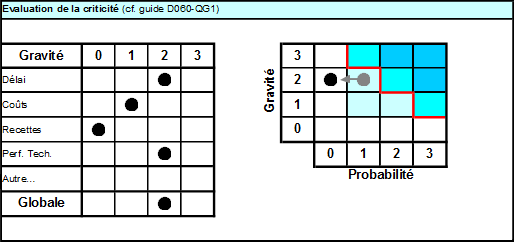
\includegraphics[width=8cm]{risque_outil.png}
		\end{figure}
		\begin{center}
			\legendeRisque
		\end{center}
	\end{frame}


% --- Risque -------------------------------------------------------------------
	\begin{frame}{\secname}
		\begin{itemize}
			\item Nouveau(x) client(s)
		\end{itemize}
		\begin{figure}
			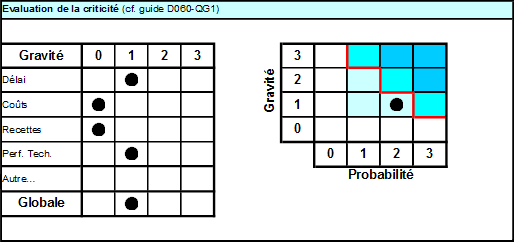
\includegraphics[width=8cm]{risque_nouveau_client.png}
		\end{figure}
		\begin{center}
			\legendeRisque
		\end{center}
	\end{frame}
	
	
% --- Risque -------------------------------------------------------------------
	\begin{frame}{\secname}
		\begin{itemize}
			\item Risque de performances
		\end{itemize}
		\begin{figure}
			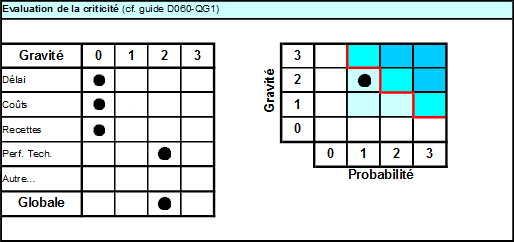
\includegraphics[width=8cm]{risque_performance.png}
		\end{figure}
		\begin{center}
			\legendeRisque
		\end{center}
	\end{frame}	
	
	
% --- Risque -------------------------------------------------------------------
	\begin{frame}{\secname}
		\begin{itemize}
			\item Risque de rendu
		\end{itemize}
		\begin{figure}
			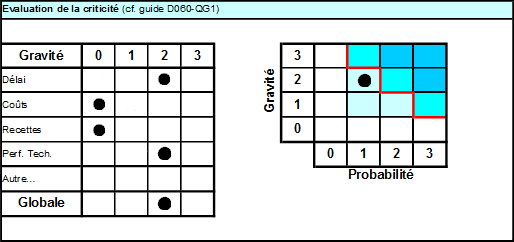
\includegraphics[width=8cm]{risque_rendu.png}
		\end{figure}
		\begin{center}
			\legendeRisque
		\end{center}
	\end{frame}


%===============================================================================
%	PAQL
%===============================================================================

\section{Plan qualit\'e logiciel}
	\begin{frame}{\secname}
		\title{\'Evaluation du livrable n°1}
		\begin{center}	
			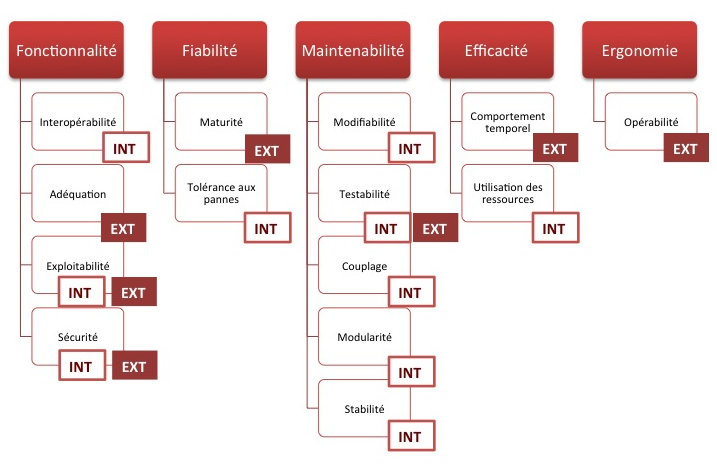
\includegraphics[width=7cm]{iso9126}
			\\\'Echelle de mesures (coefficients)\\
			\smallskip
			\footnotesize
			\begin{tabular}{|c|c|c|c|c|}
				\hline
				Fonct.(1) & Fiab.(0,1) & Maint.(1) & Effic.(0,5) & Erg.(1)\\
				\hline
				\hline
				1 & 1 & 0,5 & 1 & 1\\
				\hline
				1 & 1 & 0,5 & 0 & - \\
				\hline
				0,5 & - & 1 & - & -\\
				\hline
				0 & - & 1 & - & - \\
				\hline
				- & - & 0,5 & - & - \\
				\hline
			\end{tabular}	
		\end{center}
	\end{frame}


% --- Évaluation ---------------------------------------------------------------
	\begin{frame}{\secname}
		\begin{itemize}
			\item \'Evaluation du logiciel 
		\end{itemize}
		\begin{figure}
			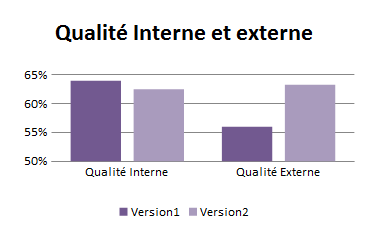
\includegraphics[width=8cm]{Images/QualiteInterneExterne.png}
		\end{figure}
	\end{frame}


% --- Évaluation ---------------------------------------------------------------
	\begin{frame}{\secname}
		\begin{itemize}
			\item Crit\`eres d'\'evaluation
		\end{itemize}
		\begin{figure}
			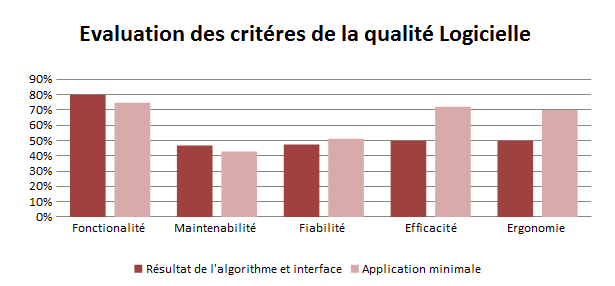
\includegraphics[width=8cm]{Images/EvaluationCriteres.png}
		\end{figure}
	\end{frame}


% --- Évaluation ---------------------------------------------------------------
	\begin{frame}{\secname}
		\begin{itemize}
			\item \'Evaluation du global logiciel 
		\end{itemize}
		\begin{figure}
			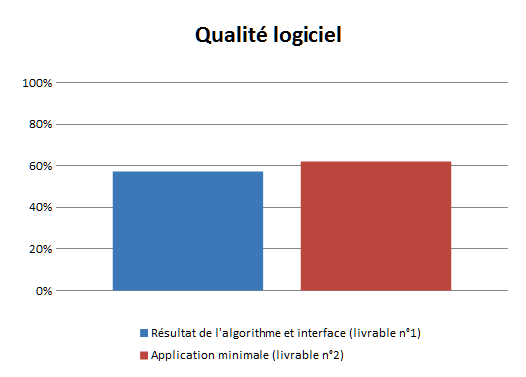
\includegraphics[width=8cm]{Images/QualiteLogicielle.png}
		\end{figure}
	\end{frame}



%===============================================================================
%	COUTS
%===============================================================================

\section{Co\^uts}
%\section{Diagramme des co\^uts}

\begin{frame}{Diagramme des co\^uts}
	\begin{figure}
		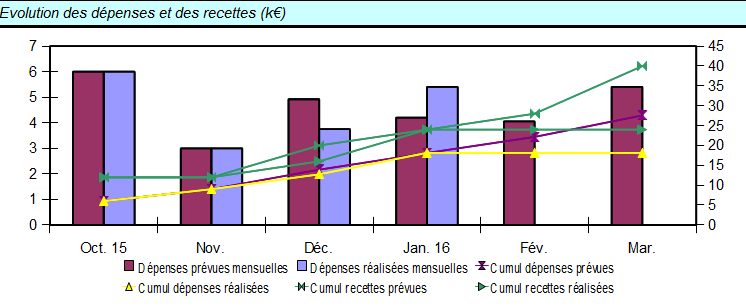
\includegraphics[height=7cm]{Images/CourbeCout.png}
	\end{figure}
\end{frame}



%===============================================================================
%	CONCLUSION
%===============================================================================

\section{Conclusion}

% --- Bilan --------------------------------------------------------------------
	\subsection{Bilan de la p\'eriode}
	\begin{frame}{\subsecname}
		\begin{itemize}
			\item Pr\'eoccupations
			\begin{itemize}
				\item Retard toujours pr\'esent
				\item Annulation probable de la t\^ache optionnelle
			\end{itemize}
		\end{itemize}
		\begin{itemize}
			\item Points forts
			\begin{itemize}
				\item Acc\'el\'eration de la g\'en\'eration et du rendu
				\item PAQL enti\`erement mis en place
				\item Retard d\^u \`a la conception en partie rattrap\'e
			\end{itemize}
		\end{itemize}
	\end{frame}


% --- Conclusion ---------------------------------------------------------------
	\subsection{\`A venir}
	\begin{frame}{\secname}
		\begin{itemize}
			\item Prochaines \'etapes
			\begin{itemize}
				\item Dessin à main lev\'ee
				\item Rentrer \'equations
				\item Gestion de donn\'ees
			\end{itemize}
		\end{itemize}
		\begin{itemize}
			\item Prochaines r\'eunions
			\begin{itemize}
				\item Audit de livraison (2 ou 3 mars)
				\item Soutenance finale (21 mars)
			\end{itemize}
		\end{itemize}
	\end{frame}



%===============================================================================
%	Remerciment
%===============================================================================

\begin{frame}{}
	\bigskip
	\bigskip
	\begin{titleblock}{}
		\begin{center}
			\smallskip
			\Large Surfaces de r\'evolution discr\`etes\\
			\medskip
			\small Revue de projet
			\smallskip
		\end{center}
	\end{titleblock}

	\bigskip
	\begin{center}
		Merci de votre attention.\\
		\medskip
		Avez-vous des questions\,?			
	\end{center}

	\bigskip
	\bigskip
	
\includegraphics[width=2cm]{../Images/logo-Xlim.png}
	\hfill
	
\includegraphics[width=2cm]{../Images/logo_univ_poitiers.png}
\end{frame}


\end{document}


